
\documentclass{beamer}


\usetheme{Warsaw}
\usecolortheme{crane}


\title{Regression Techniques}
\subtitle{Probability and Statistics for Engineers and Scientists}
\author{Steve Mazza}
\institute[Naval Postgraduate School]
{ 
    Naval Postgraduate School \\
    Monterey, CA \\
    
\includegraphics[height=3cm]{images/NPS_logo.jpg}
}
\date {SE3030, Winter/2014 \\ Quantitative Methods of Systems Engineering}
\subject{Quantitative Methods of Systems Engineering}


\begin{document}

\frame{\titlepage}


\frame{{Introduction}
  \begin{columns}[c]
    \column{.4\textwidth}
      Regression uses selected values of $x$ and observed values of $y$ in order to predict the most probable value of $y$ for any value of $x$.
    \column{.6\textwidth}
    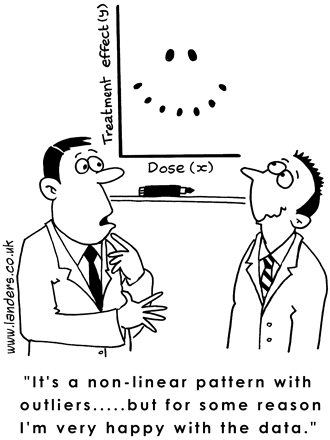
\includegraphics[scale=0.4]{images/Regression-Cartoon.png}
  \end{columns}
}


\frame{{What Is Regression?}
  Regression is a statistical process for estimating the relationships among variables.  Usually regression is used to estimate the  expected (or average) value of the dependent variable when the independent variables are fixed.  The dependent variable is a function of the independent variables.
  
  Techniques
  \begin{itemize}
  	\item simple linear regression
  	\item multiple linear regression
  	\item non-linear regression
  \end{itemize}
}


\frame{{Simple Linear Regression}
  Simple linear regression is a method of a linear regression with a single explanatory variable.  It utilizes a least squares approach to finding the best fit within the data.  It fits a \emph{straight line} through the set of $n$ points in such a way that minimizes the sum of squared residuals of the model.
  
  \begin{block}{Simple Linear Regression Model}
  	\[y_i = \beta_0 + \beta_1x_i + \epsilon_i,\; i=1\dots n\]
  \end{block}
  
  If you were to plot each of the data points on a graph, the line determined by simple linear regression would make the vertical distance from the fit line to each of the data points as small as possible.
}


\frame{{Multiple Linear Regression}
  In multiple linear regression, the response variable $y$ is modeled as a linear function of more than one input variable $x_i$.
  
   \begin{block}{Multiple Linear Regression Model}
  	\[y_i = \beta_0 + \beta_1x_i + \beta_2x_i^2 + \epsilon_i,\; i=1\dots n\]
  \end{block}
  
  While the equation is quadratic with respect to $x$, it is linear with respect to $\beta$.
  
  Due to the complexity of the calculations, multiple linear regression often utilizes linear (matrix) algebra.
}


\frame{{Non-linear Regression}
  We specify a function that relates the values of $k$ input variables and parameters $\theta$ to the response variable $y$. 
  \begin{block}{Non-linear Regression Model}
  	\[y_i = f(x_1\dots x_k; \theta_1\dots \theta_p)\]
  \end{block}
  The unknown parameters are estimated by fitting the model to the data set.  For example,
  \begin{gather*}
  	(y_1, x_{11}, \dots, x_{k1}) \\
  	\vdots \\
  	(y_n, x_{1n}, \dots, x_{kn})
  \end{gather*}
  we chose parameters to minimize the sum of squares
  \[\sum_{i=1}^n \left(y_i - f\left(x_{1i}\dots x_{ki}; \theta_1\dots\theta_p\right)\right)^2\]
}


\frame{{Questions?}
	\begin{center}
		
\includegraphics[width=.7\textwidth]{images/fin.png}
	\end{center}
}

\end{document}
